\documentclass{standalone}

\usepackage{tikz}
\usepackage{amssymb}
\usetikzlibrary{calc, positioning}
\begin{document}
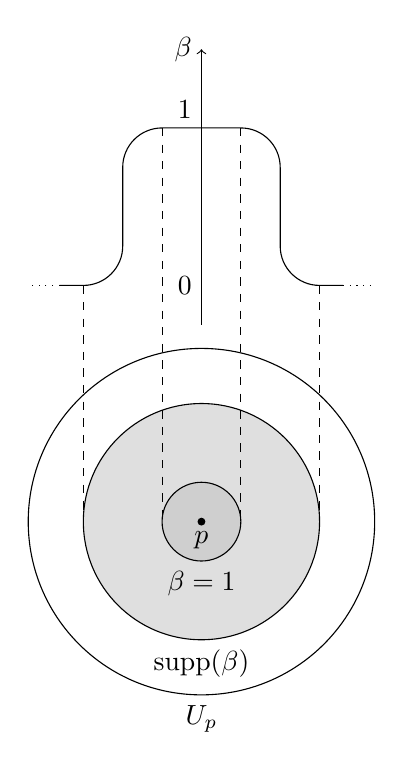
\begin{tikzpicture}
	\coordinate (p) at (0,0);

	\filldraw[fill=gray!50, fill opacity=0.5] (p) circle (1.5);
	\node[below] at ($ (p) + (0,-1.5) $) {$ \mathrm{supp}(\beta) $};
	\filldraw[fill=gray!50, fill opacity=0.5] (p) circle (0.5);
	\node[below] at ($ (p) + (0,-0.5) $) {$ \beta=1 $};

	\fill (p) circle (0.05) node[below] {$ p $};
	\draw (p) circle (2.2);
	\node[below] at (current bounding box.south) {$ U_p $};

	\begin{scope}[yshift=3cm, yscale=2]
		\draw[->] (0,-0.25) -- (0,1.5) node[left]{$ \beta $};
		\draw[rounded corners=0.5cm] (-1.8,0) -- (-1,0) -- (-1,1) -- (1,1) --
		(1,0) -- (1.8,0);
		\draw[dotted] (1.8,0) -- (2.2,0);
		\draw[dotted] (-1.8,0) -- (-2.2,0);
		\node[left] at (0,0) {$ 0 $};
		\node[above left] at (0,1) {$ 1 $};

		\coordinate (l) at (-1.5,0);
		\coordinate (r) at (1.5,0);
		\coordinate (l') at (-0.5,1);
		\coordinate (r') at (0.5,1);
	\end{scope}

	\draw[dashed] (l) to (-1.5,0);
	\draw[dashed] (r) to (1.5,0);
	\draw[dashed] (l') to (-0.5,0);
	\draw[dashed] (r') to (0.5,0);
\end{tikzpicture}
\end{document}
